%\documentclass{beamer}
\documentclass[14pt, aspectratio= 169]{beamer}
\usetheme{Copenhagen}
\usepackage[utf8]{inputenc}
\usepackage{graphicx} % Required for inserting images
\setbeamercovered{transparent}
%<1->
\setbeamertemplate{headline}{}

%%%%%%%%%%%%%%%%%%%%%%%%%%%%%%%%%%%%%%
\usepackage{listings}
\usepackage{xcolor}

% Define Python style for listings
\lstdefinestyle{python}{
    language=Python,
    basicstyle=\ttfamily\footnotesize,
    keywordstyle=\color{blue},
    commentstyle=\color{green!50!black},
    stringstyle=\color{red},
    showstringspaces=false,
    breaklines=true,
    breakatwhitespace=true,
    frame=single,
    numbers=left,
    numberstyle=\tiny\color{gray},
    captionpos=b,
    escapeinside={(*@}{@*)}
}

%%%%%%%%%%%%%%%%%%%%%%%%%%%%%%%%%%%%%%



\title{Síntesis de Redes Activas}
\subtitle{Cálculo simbólico con Python}
\author{Britez, Fabio - Corvalán, Abel \\ Ing. Ferreyra, Pablo Alejandro \\ Ing. César Reale}

\date{Facultad de Ciencas Exactas Físicas y Naturales - UNC}

\begin{document}

\maketitle


% Introducción
\begin{frame}{Introducción}
\begin{minipage}{.484\linewidth}

\includegraphics[width=.9\linewidth]{img/python.png}
\end{minipage}
\begin{minipage}{.484\linewidth}
El \textbf<1>{cálculo simbólico} en \textbf<1>{Python} se implementa para trabajar con expresiones algebraicas y funciones matemáticas en la programación.  
\end{minipage}
\end{frame}

% Objetivos
\begin{frame}{Objetivos}
\begin{itemize}
    \item Aplicar el \textbf<1>{cálculo simbólico} para la resolver ecuaciones de los circuitos propuestos en la materia Síntesis de Redes Activas.
    \item Implementar librerías necesarias para extender las capacidades del lenguaje con funciones y métodos predefinidos.
    \item Obtener expresiones matemáticas en formato LaTeX con Python.
\end{itemize}
\end{frame}

% Recomendación
\begin{frame}{Recomendación}
  Implementar el entorno de \textbf{Jupyter Notebook} para una estructura de cálculo en conjunto con representaciones y anotaciones.  
\end{frame}

% Preparación previa
\begin{frame}{Preparación previa - Instalar librerías}
Para instalar librerías \textbf{Sympy}, \textbf{Numpy}, \textbf{Math} debemos:
\begin{enumerate}
    \item Abrir un terminal \textbf{cmd}.
    \item Colocar la siguiente línea de código:
    \begin{block}{cmd}
        \begin{semiverbatim}
            pip install sympy numpy ipython
        \end{semiverbatim}
    \end{block}
\end{enumerate}
\end{frame}

% Preparación previa
\begin{frame}[fragile]{Preparación previa - Cargar librerías}
Siempre debemos cargar las librerías que usaremos en nuestro código con la siguiente estructura:
\begin{block}{Python}
\begin{semiverbatim}
import "nombre de la librería" as "expresión"
\end{semiverbatim}    
\end{block}
Si queremos implementar \textbf{sympy} lo haremos de la siguiente forma:
\begin{lstlisting}[style=python]
import sympy as sym
\end{lstlisting}
De esta forma cuando usemos un método de librería escribiremos \textbf{sym} al principio de cada llamado.
\end{frame}

% Circuito de estudio
\begin{frame}{Circuito de estudio}
    \begin{columns}
        \column{0.5\textwidth} En base al circuito que se muestra en la figura implementaremos las diferentes funcionalidades de las librerías.
        \column{0.5\textwidth} 
\begin{figure}
        \centering
        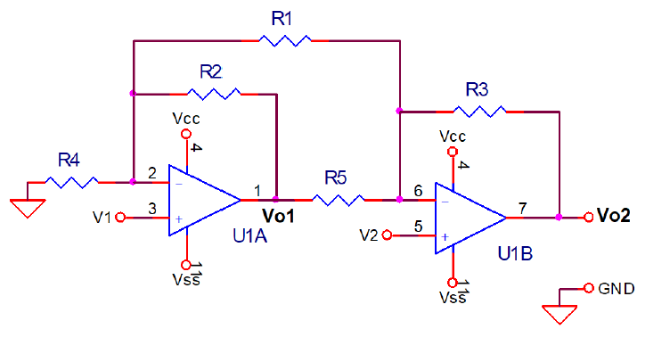
\includegraphics[width=1.0\linewidth]{img/Circuito 1.png}
        \caption{Circuito n° 1 - Laboratorio n° 1}
        \label{fig:enter-label}
    \end{figure}
        \end{columns}
\end{frame}


\begin{frame}{Items a desarrollar}
\tableofcontents
\end{frame}

\section{Cargar imágenes}
\begin{frame}[fragile]{Cargar imágenes}
Para \textbf{cargar imágenes} en nuestro programa de Python se implementa la siguiente función:

\begin{block}{Función}
Image(filename= "img/nombre de la imagen")
\end{block}
Ejemplo:
\begin{lstlisting}[style=python]
Image(filename= "img/Circuito 1.png")
\end{lstlisting}
En el campo "filename" se carga la ruta de la imágen.
\end{frame}

\begin{frame}{Expresión de salida del circuito}
Se desea obtener la respuesta de circuito respecto a $V_{1}$ y $V_{2}$.
$$ \boxed{ V_{o}= V'_{1} + V'_{2} } $$
\end{frame}

\section{Análisis del circuito}
\begin{frame}{Análisis del circuito (I)}
    \begin{columns}
        \column{0.5\textwidth} Se debe aplicar el teorema de superposición, por lo que se pasivan las fuentes $V_{1}$ y $V_{2}$ alternativamente.
        \column{0.5\textwidth}
        \begin{figure}
        \centering
        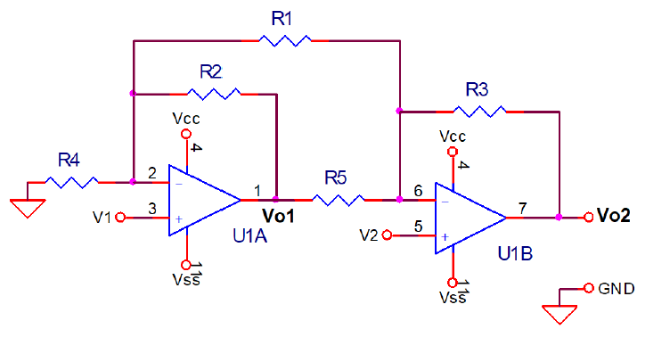
\includegraphics[width=1.0\linewidth]{img/Circuito 1.png}
        \caption{Circuito n° 1 - Laboratorio n° 1}
        \label{fig:enter-label}
    \end{figure}
    \end{columns}
\end{frame}

\begin{frame}{Análisis del circuito (II)}
    \begin{columns}
        \column{0.5\textwidth} Se estudia el caso con las siguientes condiciones:
        $$ Caso \, 1: V_{1}\neq 0V \, \, \, V_{2}=0V $$ 
        $$ Caso \, 2: V_{1}= 0V \, \, \, V_{2}\neq 0V $$
        \column{0.5\textwidth}
        \begin{figure}
        \centering
        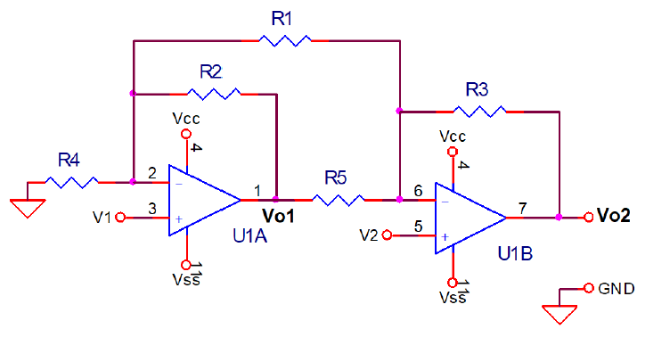
\includegraphics[width=1.0\linewidth]{img/Circuito 1.png}
        \caption{Circuito n° 1 - Laboratorio n° 1}
        \label{fig:enter-label}
    \end{figure}
    \end{columns}
\end{frame}

\begin{frame}{Análisis del circuito - Caso 1 (I)}
    \begin{columns}
        \column{0.5\textwidth} Se estudia el circuito con las siguientes condiciones:
        $$ V_{1}\neq 0V $$ $$ V_{2}=0V $$
        \column{0.5\textwidth} 
        \begin{figure}
        \centering
        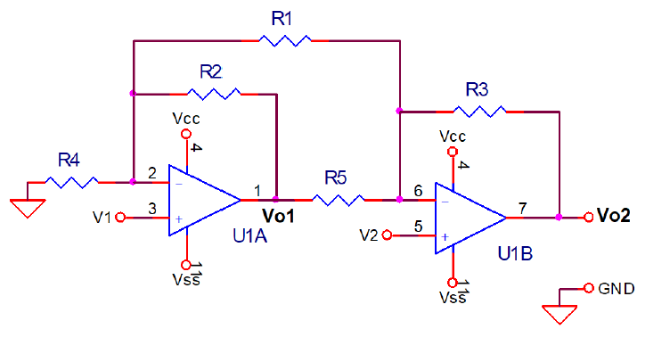
\includegraphics[width=1.0\linewidth]{img/Circuito 1.png}
        \caption{Circuito n° 1 - Laboratorio n° 1}
        \label{fig:enter-label}
    \end{figure}
    \end{columns}
\end{frame}

\section{Agregar variables simbólicas}
\begin{frame}{Agregar variables simbólicas (I)}
Se inspecciona el circuito y se detectan las variables $V_{1}, V_{2}$ y $R_{1}, R_{2}, R_{3}, R_{4}, R_{5}$. Para \textbf{agregar variables simbólicas} se escriben líneas de código con el siguiente formato:
\end{frame}

\begin{frame}[fragile]{Agregar variables simbólicas (II)}
\begin{block}{Función}
"variable en Python"= sym.symbols('"símbolo"')
\end{block}
\begin{lstlisting}[style=python]
V1,V2= sym.symbols('V_{1},V_{2}')
R1,R2,R3,R4,R5= sym.symbols('R_{1},R_{2},R_{3},R_{4},R_{5}')
\end{lstlisting}
En el lado izquierdo se tiene el nombre de cada variable dentro del programa. \\
En el lado derecho se tiene el símbolo con el que se va a mostrar en la interfaz.
Es importante escribir los símbolos del lado derecho en formato LaTeX.
\end{frame}


\begin{frame}{Análisis del circuito - Caso 1 (II)}
Las ecuaciones que modelan el amplificador para el caso 1 son las siguientes:

$$I_{R2}= \frac{V_{o1}-V_{1}}{R2}$$ 
$$I_{Rp}= \frac{V_{1}}{R_{p}}$$

Se tiene además que estas corrientes son iguales $I_{R2}=I_{Rp}$

\end{frame}

\begin{frame}[fragile]{Análisis del circuito - Caso 1 (III)}
Se agregan variables que servirán para escribir las ecuaciones de corriente mencionadas anteriormente:
\begin{lstlisting}[style=python]
Rp,Ir2,Irp,Vo1= sym.symbols('R_{p},I_{R2},I_{Rp},V_{o1}')
s_Vo1,sVo1= sym.symbols('s_Vo1,sVo1')
\end{lstlisting}
\end{frame}


\section{Escribir ecuaciones}
\begin{frame}[fragile]{Escribir ecuaciones (I)}
Para \textbf{escribir ecuaciones simbólicas} se debe escribir con el siguiente formato de código: 
\end{frame}


\begin{frame}[fragile]{Escribir ecuaciones (II)}
\begin{block}{Función}
sym.Eq('"1er miembro", "2do miembro" ')
\end{block}
\begin{lstlisting}[style=python]
equ_Ir2= sym.Eq(Ir2,(Vo1-V1)/R2)
equ_Irp= sym.Eq(Irp,(V1/Rp))
\end{lstlisting}
En el lado izquierdo se tiene el nombre del objeto de tipo \textbf{ecuación}. \\
En el lado derecho se tienen los términos de nuesta ecuación.
\end{frame}

\begin{frame}{Igualación de ecuaciones}
Como se había menciondo $I_{R2}$ y $I_{Rp}$ son equivalentes, por lo que se debe obtener el segundo miembro de cada ecuación.
\end{frame}

\section{Obtener miembro de la ecuación}
\begin{frame}{Obtener miembro de la ecuación (I)}
Para \textbf{obtener un miembro de una ecuación} se programa con la siguiente estructura:
\end{frame}

\begin{frame}[fragile]{Obtener miembro de la ecuación (II)}
Con \textbf{.lhs} se obtiene el término de la izquierda de la igualación, mientras que con \textbf{.rhs} se obtiene el término de la derecha.
\begin{block}{Función}
"nombre de la ecuación".lhs \\
"nombre de la ecuación".rhs
\end{block}
\end{frame}

\section{Igualar expresiones}
\begin{frame}[fragile]{Igualar expresiones}
Como se mencionó anteriormente se deben igualar las expresiones de $I_{R2}$ e $I_{Rp}$.

\begin{lstlisting}[style=python]
equ1= sym.Eq(equ_Ir2.rhs, equ_Irp.rhs)
\end{lstlisting}

Esto es:
$$ \boxed{ \frac{V_{o1}-V_{1}}{R_{2}}= \frac{V_{1}}{R_{P}} } $$
\end{frame}


\begin{frame}{Análisis del circuito - Caso 1 (IV)}
Ahora se quiere despejar la variable $V_{o1}$ de la ecuación \textbf{equ1}, para obtener la ganancia $V_{o1}/V_{1}$.
\end{frame}

\section{Despejar variable}
\begin{frame}[fragile]{Despejar variable}
Para despejar una variable se escribe la siguiente estructura:
\begin{block}{Función}
sym.solve("nombre de ecuación", "variable")
\end{block}
\begin{lstlisting}[style=python]
s_Vo1= sym.solve(equ1, Vo1)
\end{lstlisting}
Esta función devuelve la solución en un arreglo de tamaño n, siendo n la cantidad de soluciones.
\end{frame}


\begin{frame}[fragile]{Nueva ecuación}
Se arma una nueva ecuación para la ganancia parcial $V_{o1}/V_{1}$ a partir de la solución obtenida anteriormente.
\begin{lstlisting}[style=python]
s_Vo1= sym.Eq(Vo1/V1, s_Vo1[0]/V1)
\end{lstlisting}
\end{frame}

\section{Formatos de visualización de ecuaciones}
\begin{frame}{Formatos de visualización de ecuaciones (I)}
Para \textbf{visualizar} las ecuaciones se pueden implementar varias alternativas. Estas son:
\begin{itemize}
    \item Formato matemático en texto plano \space $sym.pprint()$
    \item Formato LaTeX \space $sym.print\_latex()$
    \item Formato simbólico
\end{itemize}
\end{frame}

% 
\begin{frame}{Formatos de visualización de ecuaciones (II)}
Se visualiza en \textbf{formato matemático en texto plano} con la función \textbf{pprint()}.
\begin{block}{Función}
sym.pprint("nombre de ecuación")
\end{block}
%Imagen
\end{frame}


\begin{frame}{Formatos de visualización de ecuaciones (III)}
Se visualiza en \textbf{formato LaTeX} con la función \textbf{print\_latex()}.
\begin{block}{Función}
sym.print\_latex("nombre de ecuación")
\end{block}
%Imagen
\end{frame}


\begin{frame}{Formatos de visualización de ecuaciones (IIV)}
Se visualiza en \textbf{formato simbólico} con la función \textbf{print\_latex()}.
\begin{block}{Función}
"nombre de ecuación"
\end{block}
Para imprimir con este formato, debe escribirse el nombre de la ecuación al final del cuadro de código.
%Imagen
\end{frame}

% 
\section{Reemplazar variables}
\begin{frame}{Reemplazar variables (I)}
Se puede \textbf{reemplazar variables} simbólicas por valores numéricos o por otras expresiones simbólicas. Se llama a esta función de la siguiente forma: 
\end{frame}

\begin{frame}{Reemplazar variables (II)}
Se hace el llamado al método \textbf{.subs()}.
\begin{block}{Función}
"nombre de ecuacion".subs("variable", "expresion o número")
\end{block}

Tenemos en nuestras ecuaciones que:
$$ R_{p}= \frac{R_{1}R_{4}}{R_{1}+R_{4}}$$

\end{frame}

\begin{frame}[fragile]{Reeemplazar variables (III)}
Para nuestro caso, queremos reemplazar la variable $R_{p}$ por su equivalente $(R1//R4)$.
\begin{lstlisting}[style=python]
s_Vo1=sVo1.subs(Rp,(R1*R4)/(R1+R4))
\end{lstlisting}
Se obtiene la siguiente expresión para la ganancia:

$$ \boxed{ \frac{V_{o1}}{V_{1}}= \frac{R_{1}+R_{4}}{R_{1}R_{4}} \Bigl(\frac{R_{1}R_{4}}{R_{1}R_{4}}+R_{2}\Bigl) } $$
\end{frame}

% 
\begin{frame}{Análisis del circuito - Caso 1 (V)}
Para obtener la expresión de la ganancia $V_{o2}/V_{o1}$ se aplica LCK.

$$ I_{R3}= I_{R5} $$

$$ \frac{V_{o2}}{R_{3}} = \frac{-V_{o1}}{R_{5}} $$

\end{frame}

% 
\begin{frame}[fragile]{Resolución ganancia $V_{o2}/ V_{o1}$ - Caso 1 (I)}
Con el siguiente fragmento de código se obtiene la ganancia $V_{o2}/V_{o1}$. 
\begin{lstlisting}[style=python]
# Cargo las variables particulares del caso de estudio.
Ir3, Ir5= sym.symbols('I_{R3}, I_{R5}')
Vo2= sym.symbols('V_{o2}')
s_Vo2, sVo2= sym.symbols('s_Vo2, sVo2')
# Escribo las ecuaciones
equ_Ir3= sym.Eq(Ir3, Vo2/R3)
equ_Ir5= sym.Eq(Ir5, -Vo1/R5)
# Igualo las expresiones Ir3 e Ir5.
equ2= sym.Eq(equ_Ir3.rhs, equ_Ir5.rhs)
# Resuelvo sistema, se obtiene solucion en formato matriz.
s_Vo2= sym.solve(equ2, Vo2)
# Obtengo solucion
sVo2= sym.Eq(Vo2/Vo1, s_Vo2[0]/Vo1)
\end{lstlisting}

\end{frame}

% 

\begin{frame}[fragile]{Resolución ganancia $V_{o2}/ V_{o1}$ - Caso 1 (II)}
\begin{lstlisting}[style=python]
#Formula en formato de texto plano.
sym.pprint(sVo2)
#Formula en formato latex
print('Formula en formato LaTex: ')
sym.print_latex(sVo2)
#Formula en formato simbolico
sVo2
\end{lstlisting}
\end{frame}

% 

\begin{frame}{Resolución ganancia $V_{o2}/V_{o1}$ - Caso 1 (III)}
Se obtiene la siguiente expresión para la ganancia $V_{o2}/V_{o1}$.
$$ \boxed{ \frac{V_{o2}}{V_{o1}}= -\frac{R_{3}}{R_{5}} } $$
\end{frame}

% 
\begin{frame}{Resolución - Caso 1 (I)}
Se obtiene la ganancia del circuito para el caso 1 ($V_{1}\neq 0V \, \, \, V_{2}=0V$)

$$ \boxed{ A_{V1} = - \frac{R_{3} \left(R_{1} R_{4} + R_{2} \left(R_{1} + R_{4}\right)\right)}{R_{1} R_{4} R_{5}} } $$

$$ \boxed{ V_{o}= -3 V_{1} } $$
%$$ Caso \, 2: V_{1}= 0V \, \, \, V_{2}\neq 0V $$
\end{frame}


%%%% Caso 2 
\begin{frame}{Análisis del circuito - Caso 2 (I)}
    \begin{columns}
        \column{0.5\textwidth} Se estudia el circuito con las siguientes condiciones:
        $$ V_{1}= 0V $$ $$ V_{2}\neq0V $$
        \column{0.5\textwidth}
        \begin{figure}
            \centering
            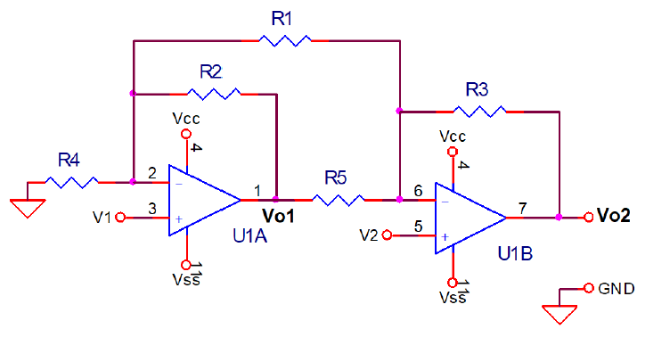
\includegraphics[width=1.0\linewidth]{img/Circuito 1.png}
            \caption{Circuito n° 1 - Laboratorio n° 1}
            \label{fig:enter-label}
        \end{figure}
    \end{columns}
\end{frame}

\begin{frame}{Análisis del circuito - Caso 2 (II)}
Las ecuaciones que modelan el amplificador para el caso 2 son las siguientes:

$$I_{R1} = - \frac{V_{2}}{R_{1}}$$ 
$$I_{R2} = \frac{V_{o1}}{R_{2}}$$

Se tiene además que estas corrientes son iguales $I_{R1}=I_{R2}$
\end{frame}

\begin{frame}[fragile]{Script - Caso 2 (I)}
Se realiza el siguiente script:
\begin{lstlisting}[style=python]
# Cargo las variables particulares del caso de estudio.
Ir1, R= sym.symbols('I_{R1}, R')
# Escribo las ecuaciones de Ir1 e Ir2.
equ_Ir3= sym.Eq(Ir2, Vo1/R2)
equ_Ir5= sym.Eq(Ir1, -V2/R1)
# Igualo las expresiones Ir3 e Ir5.
equ2= sym.Eq(equ_Ir3.rhs, equ_Ir5.rhs)
sym.pprint(equ2)
# Resuelvo sistema, se obtiene solucion en formato matriz.
s_Vo1= sym.solve(equ2, Vo1)
# Obtengo solucion
sVo1= sym.Eq(Vo1, s_Vo1[0])
\end{lstlisting}
\end{frame}


% 
\begin{frame}[fragile]{Script  - Caso 2 (II)}
Para la segunda etapa se tiene:
\begin{lstlisting}[style=python]
# Cargo las variables particulares.
Vx, Vo= sym.symbols('V_{x}, V_{o}')
# Nodo Vx es igual a la salida Vo1
Vx= sVo1.rhs
# Se aplica LCK
Vop= sym.Eq(((Vo2-V2)/R3), ((V2-Vx)/R5)+(V2/R1))
# Se normaliza el valor de las resistencias
s_Vo= Vop.subs({R1: R, R2: R, R3: R, R4: R, R5: R})
# Se despeja Vo.
sVo2= sym.solve(s_Vo, Vo2)
# Se arma la ecuación de Vo
s= sym.Eq(Vo, sVo2[0])
\end{lstlisting}
\end{frame}


\begin{frame}{Resolución Caso 2 (I)}
Se obtiene la siguiente expresión del circuito para el caso 2 ($V_{1}= 0V \, \, \, V_{2}\neq 0V$)

$$ \boxed{ V_{o}= 4 V_{2}} $$
\end{frame}

% 
\section{Resolución del circuito completo}
\begin{frame}{Resolución del circuito completo}

Finalmente sumando las respuestas del circuito aplicando el teorema de superposición:

$$ \boxed{ V_{o}= -3 V_{1} + 4 V_{2} } $$

\end{frame}

\end{document}
